\documentclass[12pt]{article}
\title{Project 3}
\author{Eirik Ramsli Hauge\\
Joakim Kalsnes
}
\date{\today}

\usepackage{amsmath}
\DeclareMathOperator*{\argmin}{argmin}
\usepackage{bm}
\usepackage{xcolor}
\usepackage{hyperref}
\usepackage[english]{babel} 
%\usepackage{fullpage} 
\usepackage{amsfonts} 
\usepackage{amssymb} 
\usepackage{verbatim} 
 
\usepackage{color} 
\usepackage{setspace} 
\usepackage{blindtext}
\usepackage{epstopdf} 
\usepackage{braket}

\usepackage{cite} 
\usepackage{caption}
\usepackage{subcaption}
\usepackage{upgreek}
\usepackage{array,multirow}
\usepackage{pdfpages}

\usepackage{graphicx} 
\usepackage{float}

\usepackage{nameref}
\usepackage{hhline}
\usepackage{xtab}
\usepackage{booktabs, makecell, longtable}
\usepackage{lscape}

\numberwithin{figure}{section}

\newcommand{\husk}[1]{\color{red} #1 \color{black}}
\newcommand{\sjekk}[1]{\color{violet} #1 \color{black}}

\bibliographystyle{unsrt}

\begin{document}
\maketitle
\begin{abstract}
In this paper we are provided with credit card default data and will use three different methods to make a classification model. We will use logistic regression, neural net and random forrest models. All these models are imported from commonly known libraries and will not be written by ourselves. Through this paper we want to compare these models against each other and to those found by Yeh and Lien \cite{yeh}. It is believed that the random forrest model will be able to compete with their best model, the neural net. We found that our logistic regression and neural net were equal to theirs, and that our random forrest did not perform better. This is probably due to poor choice of parameters for the random forrest and for future works this should be looked further into.
\end{abstract}
\section{Introduction}
Throughout this course we have studied numerous different machine learning methods for both regression and classification analysis. In this project we will use the classifications methods we have learned on real-life data. We will study the credit card data set presented at the site of UCI \cite{UCI}. The data set consists of 25000 credit card observations taken in 2005 from an important bank in Taiwan. In order to get more costumers, banks in Taiwan lowered the requirements for credit card approval. Cardholders, at the same time, overused their credit cards and accumulated heavy debts.\\
This study will try to use information such as business financial statement, repayment records and personal information (gender, age, education, marital status) to predict whether or not the costumer will be able to repay their credit card debt. To make our predictions, we will use logistic regression, neural networks and random forest. The calculations will be performed using the Scikit-Learn and Keras packages. The credit card data set has previously been studied by Yeh and Lien \cite{yeh}, so it will be natural to compare our results to theirs. However, random forests was not tested by Yeh and Lien, so it will be interesting to see how these results compare to the other classification methods.\\


\section{Theory}
For this project we are going to use logistic regression, neural networks and random forest to analyse the credit card example. Logistic regression and neural networks were described in project 2 (\cite{project2}). This theory section will therefore focus on random forest, starting with a presentation of decision trees.
\subsection{Decision Trees}
This section will follow closely the description of decision trees in chapter 6 of Geron's book \cite{Geron}.\\
Decision trees is a type of Machine Learning algorithm that can be used for both regression and classification. They are easy to interpret and intuitive in the way the algorithm is constructed. As we will see in the next section, they are the fundamental components of random forests. To understand how decision trees work, we start by looking at an example. Figure \ref{figT:iris_tree} shows a decision tree made on the classic iris dataset using Scikit-Learn (taken from Géron p. 170 \cite{Geron}). The goal of the model is to classify an iris flower. When we have a new flower, we start at the \textit{root node} (depth=0) and ask if the petal length is smaller than 2.45 cm. If it is, we move down the tree to the left child node (depth=1, left). In this example, it is a leaf node, that is it does not have any children nodes. From this lead node we see that the decision tree predicts that the flower is and Iris-setosa (class=setosa). If the petal length is longer than 2.45 cm we move to the root's right child node (depth=1, right). This is not a leaf node, so it asks a new question: is the flower's petal width smaller than 1.75 cm? If it is, then the flower is most likely of class Versicolor. If it is not, it is most likely of class Virginica.\\ 
\begin{figure}[H]
\centering
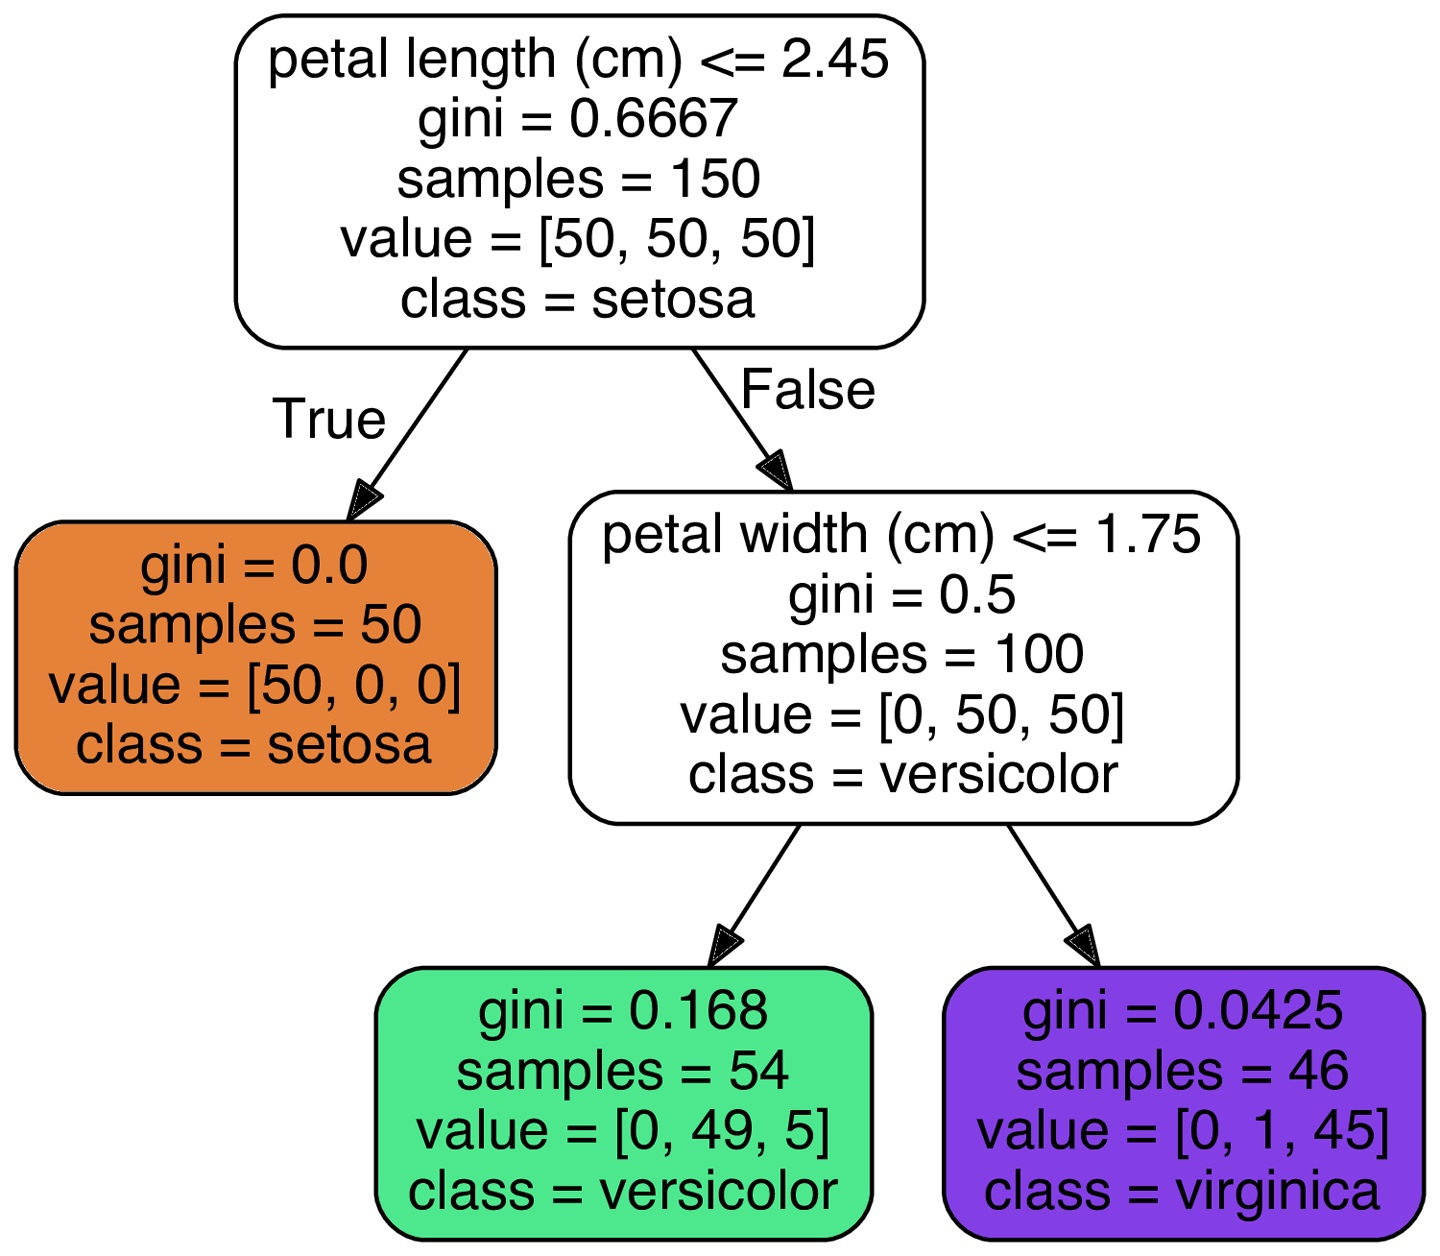
\includegraphics[width=0.8\linewidth]{decision-tree-iris.jpg}
\caption{Iris Decision Tree}
\label{figT:iris_tree}
\end{figure}
\noindent
A node's \textit{samples} attribute counts how many training instances it applies to. For example, in Figure \ref{figT:iris_tree}, 50 training instances have a petal length smaller than 2.45 cm. The \textit{value} attribute tells us how many training instance of each class this node applies to. For example, the bottom left applies to 0 Iris-Setosa, 49 Iris-Versicolor and 5 Iris-Virginica. The \textit{class} gives the most likely class, i.e. the class with the highest count in \textit{value}. We can also get the probability of each class as an output (not shown in Figure \ref{figT:iris_tree}). The probability is simple the ratio of class instances among the training instances in the given node. For example in (depth 2, left), the probabilities are: p(class=setosa) = 0/54, p(class=versicolor) = 49/54 and p(class=virginica) = 5/54. Finally, a node's \textit{gini} attribute measures its \textit{impurity}. A node is "pure" ($gini=0$) if all training instances it applies to belong to the same class, e.g. (depth 1,left) in figure \ref{figT:iris_tree}. The gini score, G$_i$, is calculated using the following equation:
\begin{equation}
G_i = 1 - \sum_{k=1}^{n}{p_{i,k}}^2,
\label{eqT:gini_score}
\end{equation}
where $p_{i,k}$ is the ratio of class $k$ instances among the training instances in the $i^{th}$ node. As an example, the gini score of (depth 2, right) is: $1-(0/46)^2-(1/46)^2-(45/46)^1 \approx 0.0425$. \\ \\
To train, or "grow", decision trees, Scikit-Learn uses the \textit{Classification and Regression Tree} (CART) algorithm. The algorithm first splits the training set in two subsets using a single feature $k$ and a threshold$t_k$. To choose $k$ and $t_k$, the algorithm searches for the pair $(k, t_k)$ that produces the purest subsets. The cost function to minimize is given by the following equation:
\begin{equation}
J(k,t_k) = \frac{m_{left}}{m}G_{left}\ +\ \frac{m_{right}}{m}G_{right},
\label{eqT:CART_cost}
\end{equation}
where $G_{left/right}$ measures the impurity of the left/right subset and $m_{left/right}$ is the number of instances in the left/right subset. The Gini impurity measure (equation \ref{eqT:gini_score}) is used by default, but one can also use entropy impurity defined by:
\begin{equation}
H_i = - \underbrace{\sum_{k=1}^{n} p_{i,k}log(p_i{i,k})}_{p_{i,k}\neq0},
\label{eqT:entropy_cost}
\end{equation}
where $p_{i,k}$ is the same as in equation \ref{eqT:gini_score}. Once the algorithm has split the training set in two subsets, it splits the subsets using the same logic, then the sub-subsets and so on. The algorithm will stop when it cannot find a split that reduces the impurity or when it reaches the maximum depth, which is a hyperparameter set by the user. \\ \\
Decision trees make very few assumptions about the training data. If no constrain is set on the algorithm, it will likely adapt the tree structure very well to the training data. This will however most likely lead to overfitting, and the tree will generalize poorly to test data. To avoid overfitting, we therefore need to restrict, regularize, the decision tree. One way is by restricting the maximum depth of the tree, where a lower maximum depth reduces the risk of overfitting. Other parameters that restrict the shape of the decision tree is:\\
$\bullet$ Minimum number of samples a node must have before it can be split.\\
$\bullet$ Minimum number of samples a leaf node must have (absolute number or fraction of total instances).\\
$\bullet$ Maximum number of leaf nodes.\\
$\bullet$ Maximum number of feature that are evaluated for splitting at each node.\\ \\
We will only use decision tress and random forests for classification, but we mention briefly here that can be used for regression as well. The algorithm, and hence the decision trees, are very similar to the classification case. The regression prediction will simply be the average value of the training instances in the leaf node you end up in. The splitting is now done in way that minimizes the mean squared error (MSE) rather than the impurity.\\ \\
The main issue with decision trees is that are very sensitive to small variations in the training data. Just removing or adding one sample, may change the tree completely. In addition, since the Scikit-Learn model is stochastic we might get very different models on the same training set.  Random forests limits this instability by averaging over many trees.\\ \\

\subsection{Random Forests}
This section is heavily based on chapter 7 about ensemble learning and random forests in Géron's book \cite{Geron}.\\
The idea behind random forests is simple: You train a group of decision trees, each on a different random subset of the training set. To make predictions, you obtain the predictions from all individual trees, then predict the class that gets the most votes. Random forests is an \textit{Ensemble method}, where an \textit{ensemble} in machine learning is  a group of predictors.\\ \\
When making the prediction, there are different ways of counting the votes. One can use either \textit{hard voting} or \textit{soft voting}. Hard voting is the most straightforward method where you just count the number of predictors that predict each class, and choose the class that got the most votes. In soft voting, we use the probability of each class. The class probabilities are found from averaging the predicted probability over all individual predictors. To predict the class, we then use the class with the highest class probability. Soft voting gives more weight to highly confident votes, and therefore often achieves higher performance than hard voting.\\ \\
Like discussed above, random forest is an ensemble of decision trees. The trees are usually trained using the bagging method, or sometimes pasting. Both of these methods use the same training algorithm for every predictor, but trains them on different random subsets of the training set. Bagging uses sampling with replacement (bootstrap), while pasting samples without replacement. The bias is higher for each individual predictor than if it were trained on the complete training set, but aggregation reduces both bias and variance. The result is generally a similar bias but a lower variance for the ensemble compared to a predictor trained on the original training set. This means that the ensemble's (random forest) prediction will generalize better than the single decision tree's prediction.\\
In addition to sampling training instances, the random forest algorithm samples features. Instead of searching for the very best feature when splitting a node, it searches for the best feature among a random subset of features. This also results in higher bias and lower variance, making a more generalizable and overall better model.\\ \\
In our project we will use the \textit{RandomForestClassifier} class from Scitkit-Learn. When using \textit{RandomForestClassifier}, we can adjust all the hyperparameters described in the Decision Tree section, as well as hyperparameters controlling the sampling.\\
A great quality of random forest is that they make it easy to measure the relative importance of each feature. "Scikit-Learn measures importance by looking at how much the tree nodes that use the feature reduce impurity on average (across all trees in the forest). More precisely, it is a weighted average, where each node's weight is equal to the number of training samples that are associated with it." \cite{Geron}[p. 192] 
\subsection{Gain curves}
Gain curves are used extensively (e.g. figure \ref{figR:LogReggain}) throughout this paper and must therefore be explained here. Yeh et al. \cite{yeh} has a good explenation, but wrongly names it lift chart. These charts are similar and related, but not quite the same. The quote below is therefore corrected in parentheses where necessary:
"In the lift chart (gain chart), the horizontal
axis represents the number (percentage) of total data. The vertical
axis shows the cumulative number of target data (in percentage). There are
three curves – model curve, theoretically best
curve (Optimal), and diagonal baseline curve, in the lift chart. The greater the area between the model curve and the baseline curve, the better the model. Area
ratio is defined as:
\begin{equation}
\text{Area ratio} = \frac{\text{Area between model curve and baseline curve}}{\text{Area between theoretically best curve and baseline curve}}
\end{equation}
In this paper, the model curve will be named "Class 1".
\section{Experimental}
The script used in all calculations presented in this paper can be found at the github repository \cite{github}. In the \texttt{src} folder one will find the file \texttt{main.py}. By running this file and a set of inputs, one can run different instances of the script. An overview of the different input arguments is presented in table \ref{tabE:sysargv}:
\begin{table}[H]
\centering
\begin{tabular}{c|p{10cm}}
Argument & Effect \\ \hline
b & Runs the logistic regression classifier \\ \hline
b Optimal & Runs the logistic regression classifier for different values of $\lambda$ \\ \hline
c & Runs the neural network classifier with the standard network \\ \hline
c Deep & Runs a neural network classifier which is made extra deep (many layers with few neurons) \\ \hline
c Wide & Runs a neural network classifier which is made extra wide (few layers with many neurons) \\ \hline
d & Runs a random forrest classifier \\ \hline
d Optimal & Runs the random forrest classifier for different parameters \\ \hline
\end{tabular}
\caption{The different input arguments and their effect when running \texttt{src/main.py}}
\label{tabE:sysargv}
\end{table}
Other features such as grid searching to find the optimal variables were changed directly in the script. This is not the ideal way to do it, but was chosen to save time.
Before any data is processed it is read from a \texttt{.csv}-file which can be found at \cite{UCI} where the attribute information also can be found.
\section{Results}
The results are all made up of two smaller sections for each method of classification. Firstly, we find the optimal parameters and then we apply those parameteres to find the optimal gain-curve and area ratio.

\subsection{Logistic Regression}
Finding the optimal logistic regression we ran our classifier for different values of $\lambda$. The resulting accuracy and area ratios can be found in figure \ref{figR:LogRegParam}:
\begin{figure}[H]
\centering
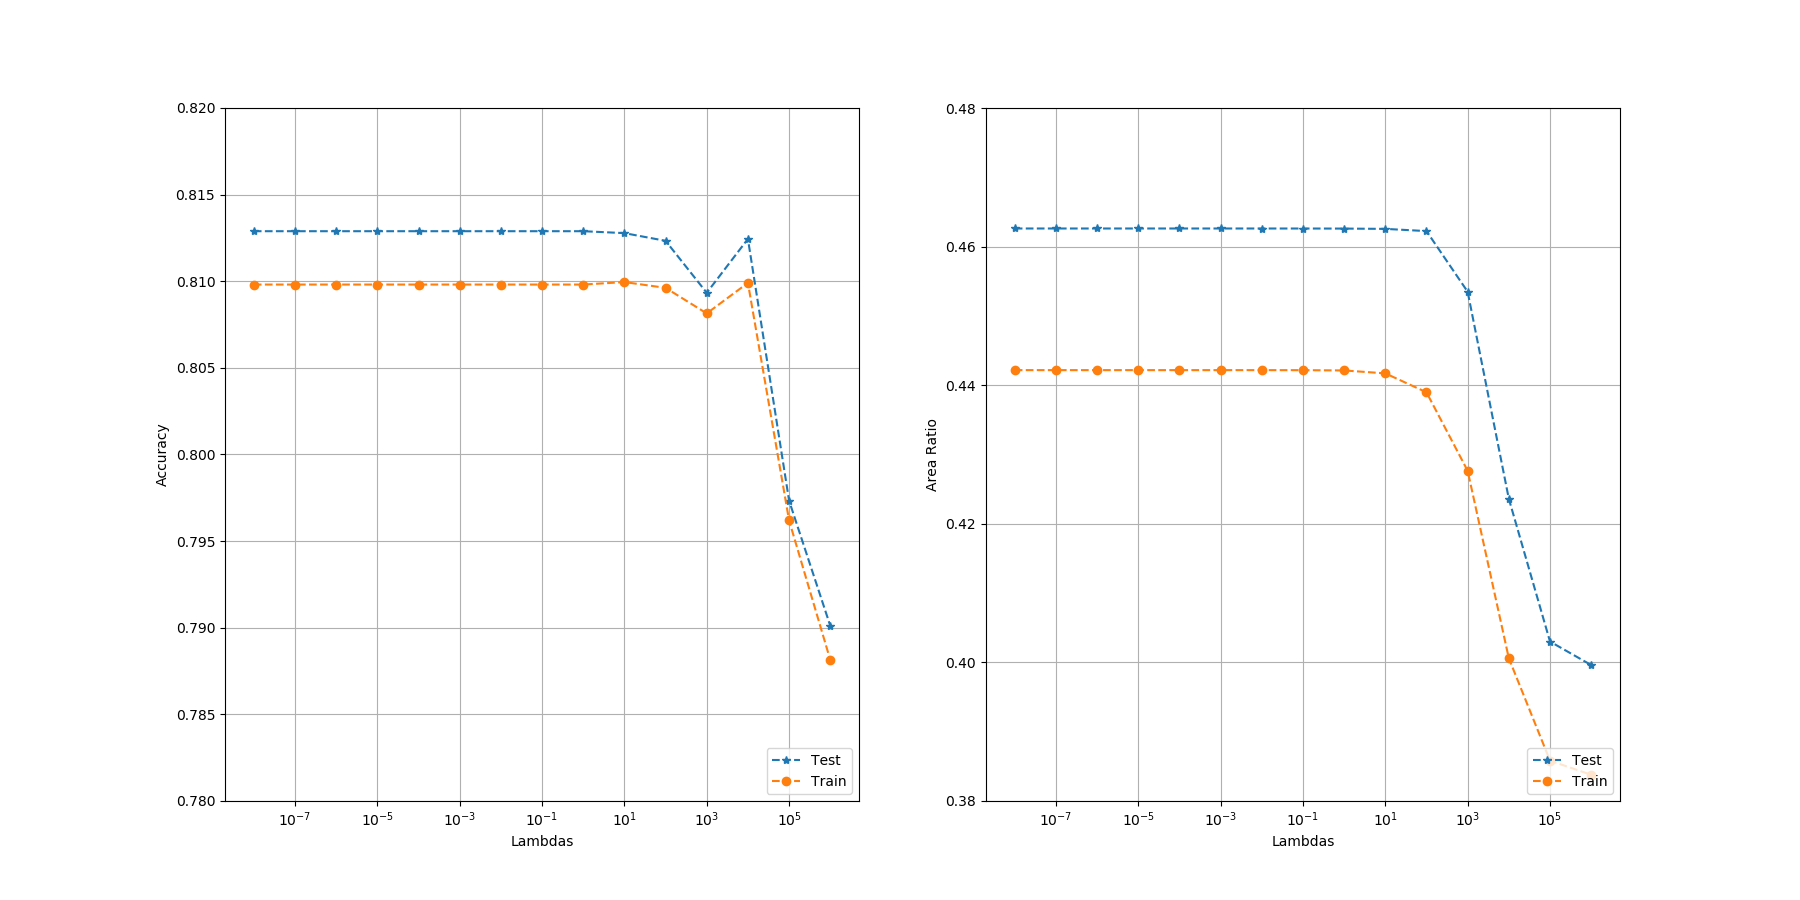
\includegraphics[scale=0.38]{../figures/LogRegOpti.png}
\caption{Accuracy as a function of $\lambda$ value for our Logistic Regression model}
\label{figR:LogRegParam}
\end{figure}
As we can see, there is little difference in the lower values, but for the higher values it the acccuracy and the area ratio drops. We therefore opted for $\lambda = 1\cdot 10^{-5}$.\\ \\
With the $\lambda$ parameter set, we calculated the gain-curve displayed in figure \ref{figR:LogReggain}. The area ratios can be found in table \ref{tabR:arearatio}.
\begin{figure}[H]
\centering
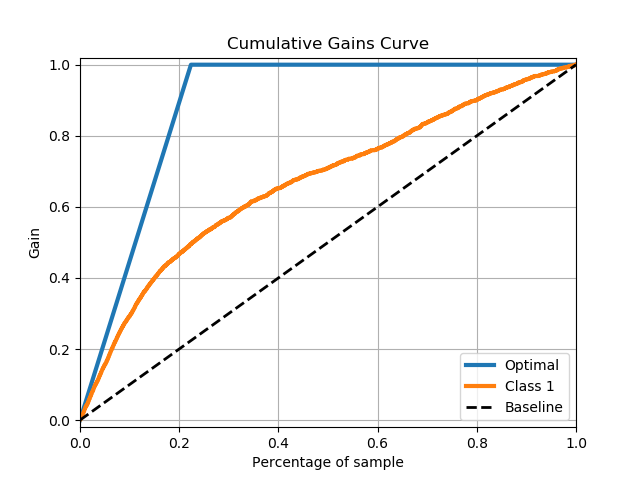
\includegraphics[scale=0.8]{../figures/gain-LogReg.png}
\caption{Gain chart for our Logistic Regression}
\label{figR:LogReggain}
\end{figure}
\subsection{Neural Network}
To find the optimal settings for our neural network many parameters were tweaked before we found the best set. Color plots in figure \ref{figR:cpMomDec} - \ref{figR:cpEplr} displays the accuracy of two and two parameters compared against each other.
\begin{figure}[H]
\centering
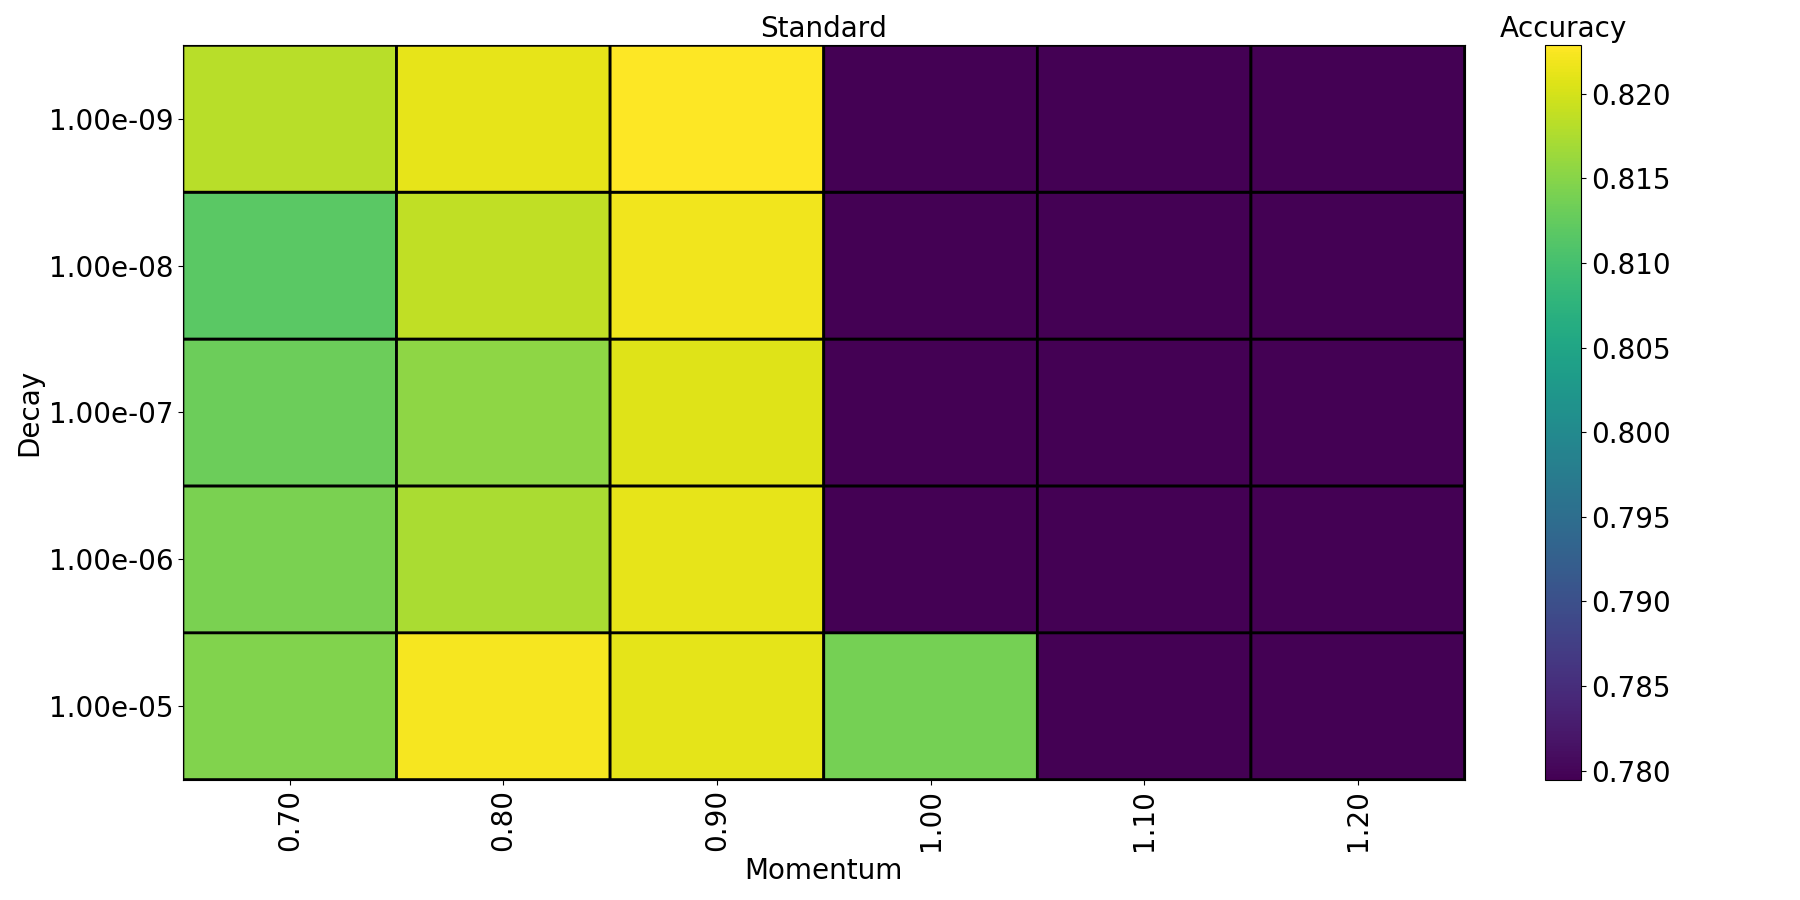
\includegraphics[scale=0.25]{{../figures/Standard-Momentum-Decay-1.00e-09-Accuracy-mini0.78-maxi0.82}.png}
\caption{A comparison of the Neural Net accuracy between the parameters Momentum and Decay.}
\label{figR:cpMomDec}
\end{figure}

\begin{figure}[H]
\centering
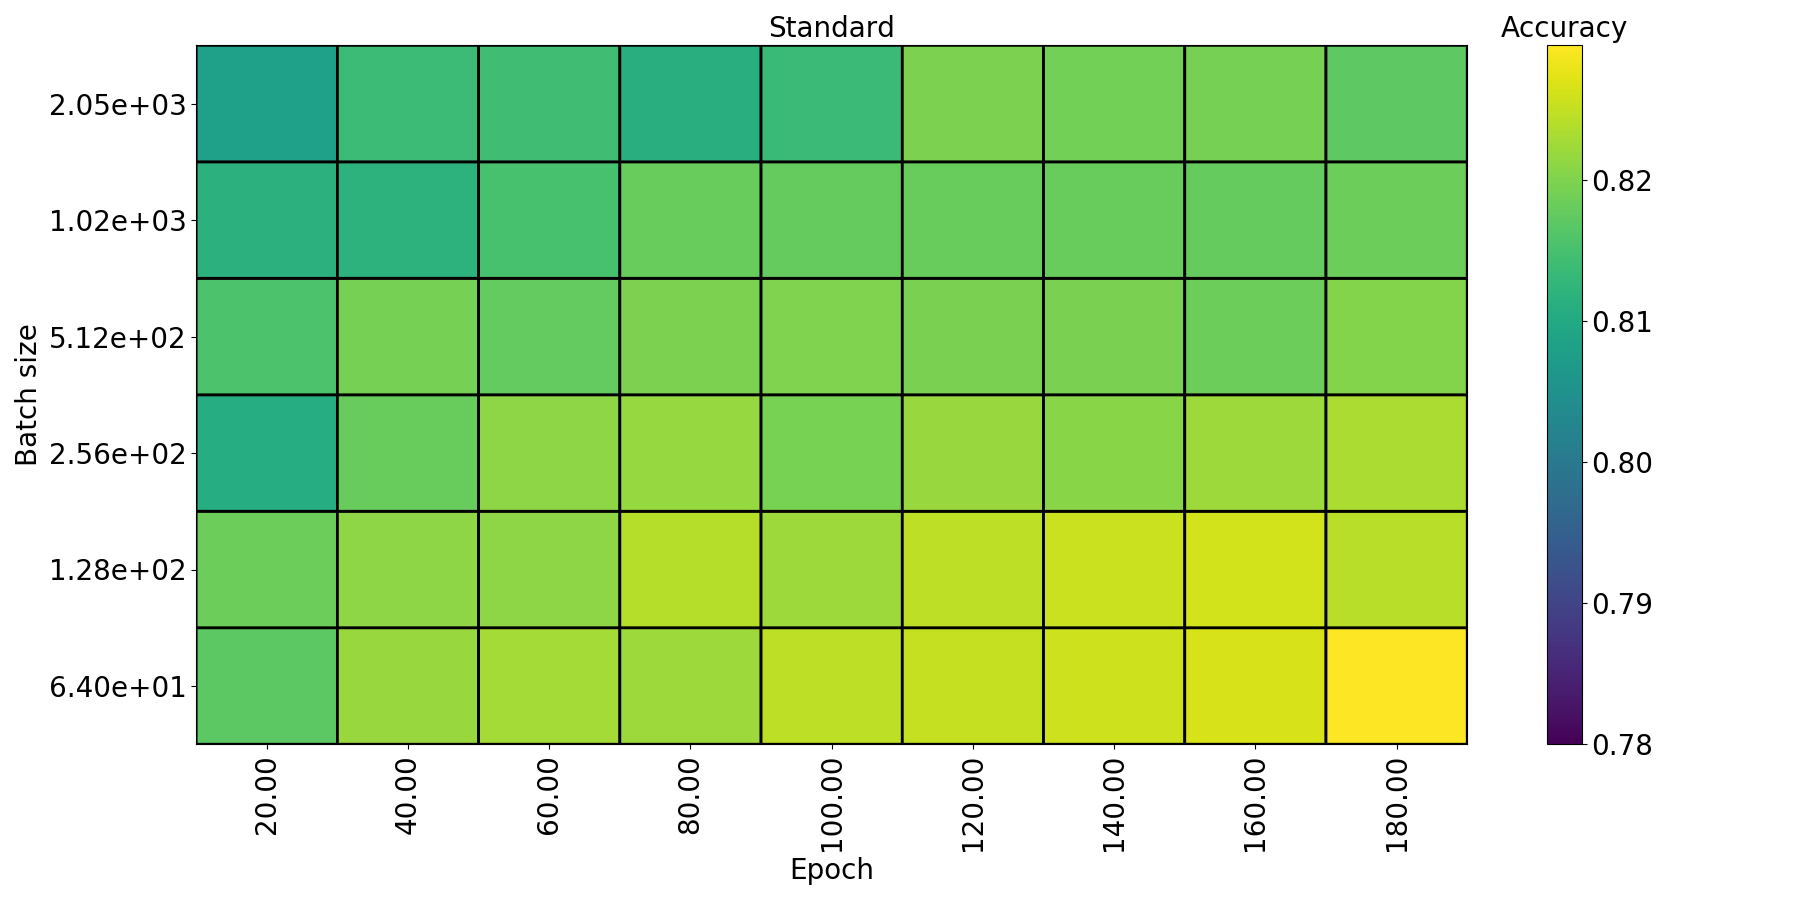
\includegraphics[scale=0.25]{{../figures/Standard-Epoch-Batchsize-2.05e+03-Accuracy-mini0.78-maxi0.83}.png}
\caption{A comparison of the Neural Net accuracy between the parameters Epoch and Batch size.}
\label{figR:cpEpBS}
\end{figure}

\begin{figure}[H]
\centering
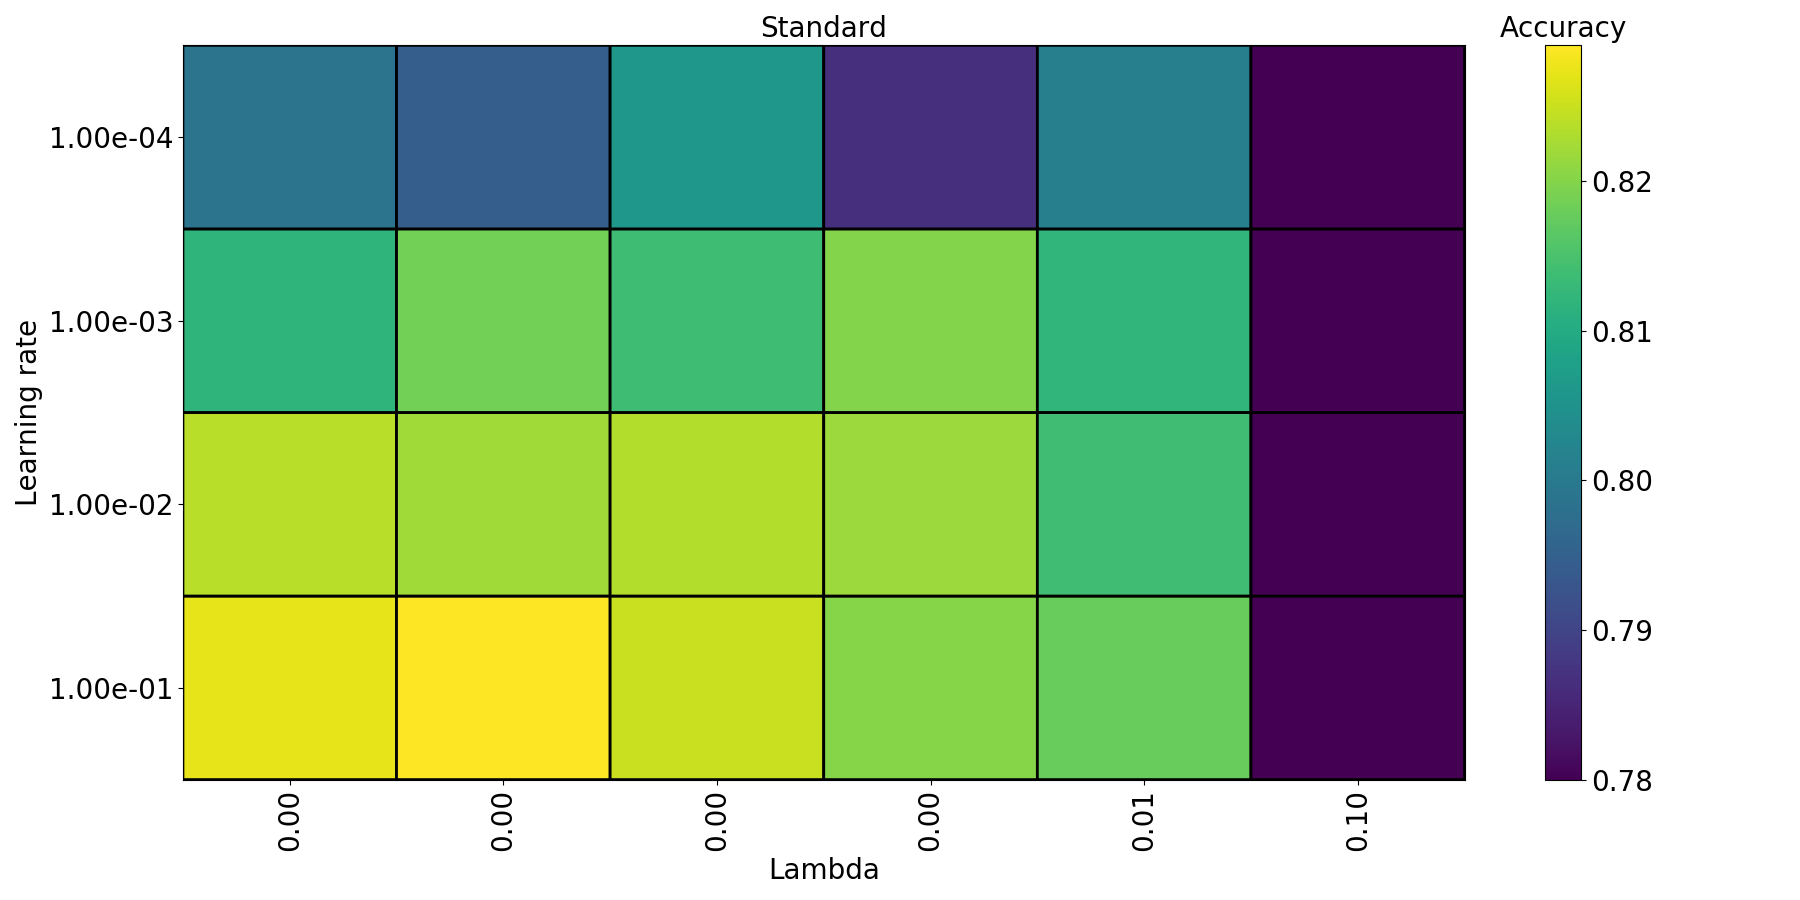
\includegraphics[scale=0.25]{{../figures/Standard-Lambda-Learningrate-1.00e-04-Accuracy-mini0.78-maxi0.83}.png}
\caption{A comparison of the Neural Net accuracy between the parameters $\lambda$ and learning rate.}
\label{figR:cplmblr}
\end{figure}

\begin{figure}[H]
\centering
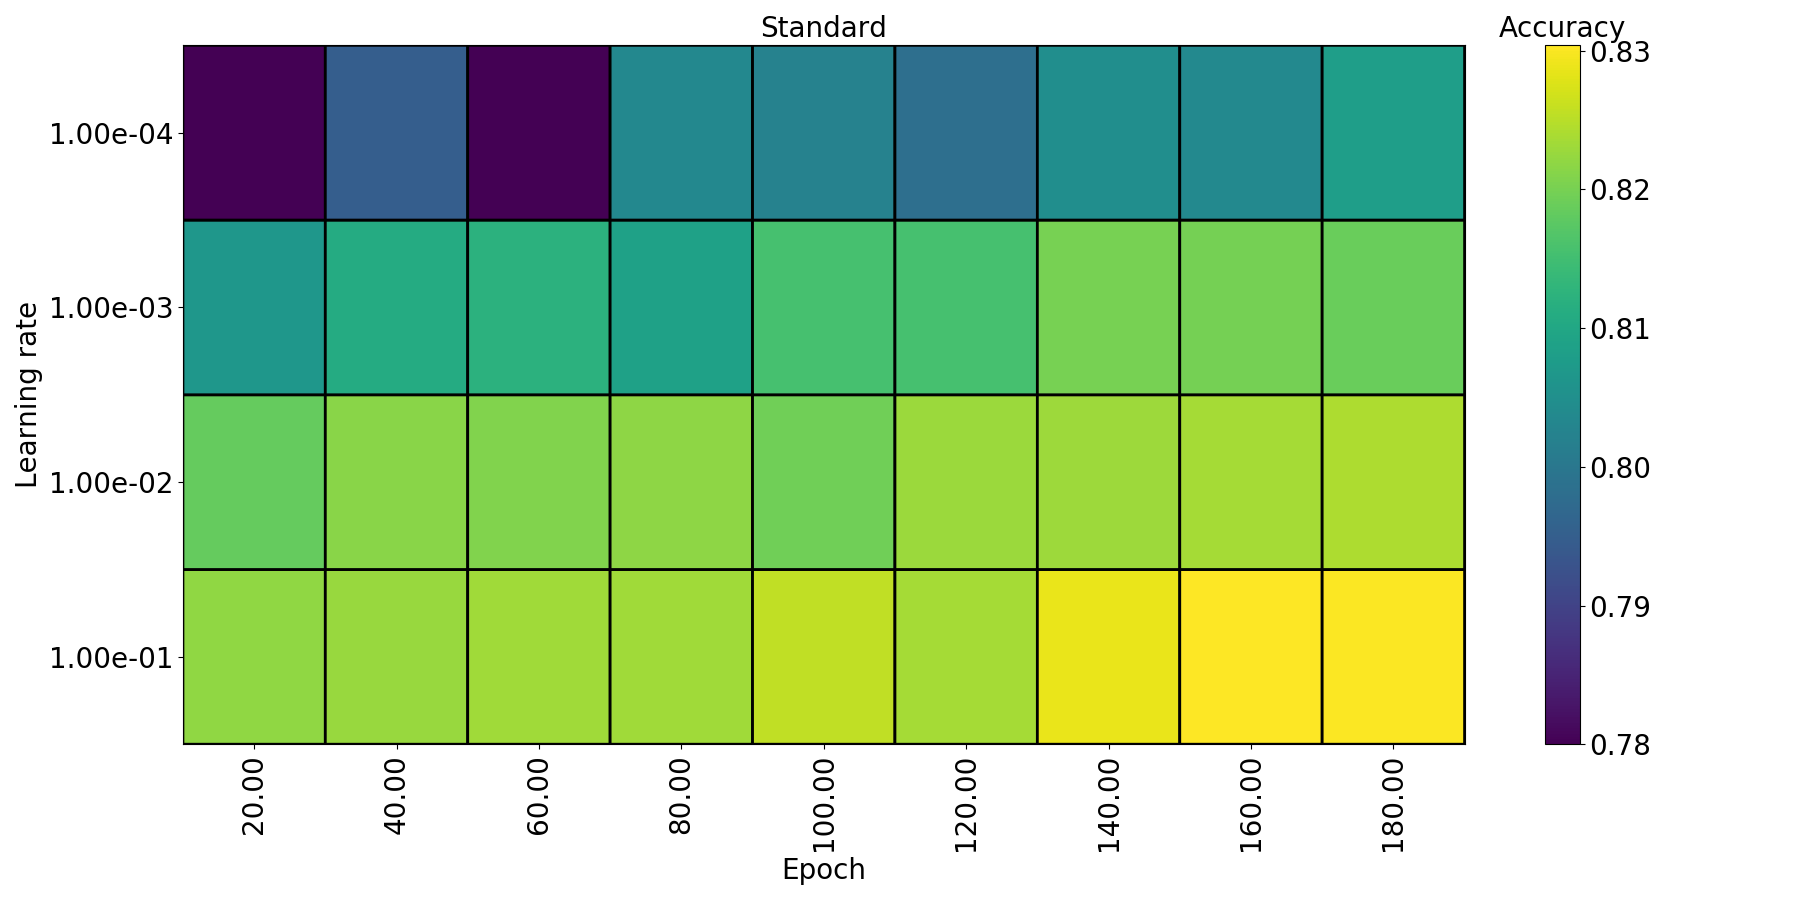
\includegraphics[scale=0.25]{{../figures/Standard-Epoch-Learningrate-1.00e-04-Accuracy-mini0.78-maxi0.83}.png}
\caption{A comparison of the Neural Net accuracy between the parameters epoch and learning rate.}
\label{figR:cpEplr}
\end{figure}

It was also found that the net type "Standard" gave the highest accuracy. \\ \\

Thus, as a compromise between computational time and accuracy, the parameteres in table \ref{tabR:parameters} were chosen:
\begin{table}[H]
\centering
\begin{tabular}{c|c}
Parameter & Value \\ \hline
Net type & Standard \\
Momentum & 0.9 \\
Decay & $1.0 \cdot 10^{-8}$ \\
$\lambda$ & $1.0 \cdot 10^{-5}$ \\
Learning rate & 0.1 \\
Epochs & 140 \\
Batch size & 256 \\ \hline
\end{tabular}
\caption{Parameters chosen for our neural network}
\label{tabR:parameters}
\end{table}
With these parameters we ran our neural network on the data provided which resulted in the gain plot in figure \ref{figR:nngain} and the area ratio presented in table \ref{tabR:arearatio}.
\begin{figure}[H]
\centering
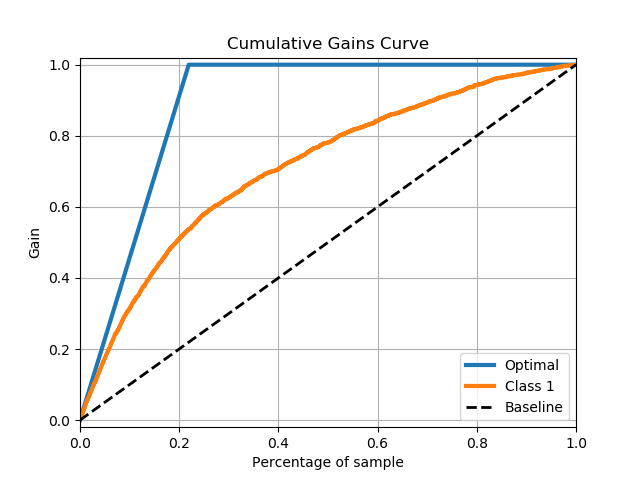
\includegraphics[scale=0.8]{../figures/gain-NN.png}
\caption{Gain chart for our Neural Network}
\label{figR:nngain}
\end{figure}
\subsection{Random Forrest}
Similarily, we found the optimal parameters for a random forrest (figures \ref{figR:randomforrest1}- \ref{figR:randomforrest4}) and produced the gain plot presented in figure \ref{figR:randomforrest}. \\ \\
\begin{figure}[H]
\centering
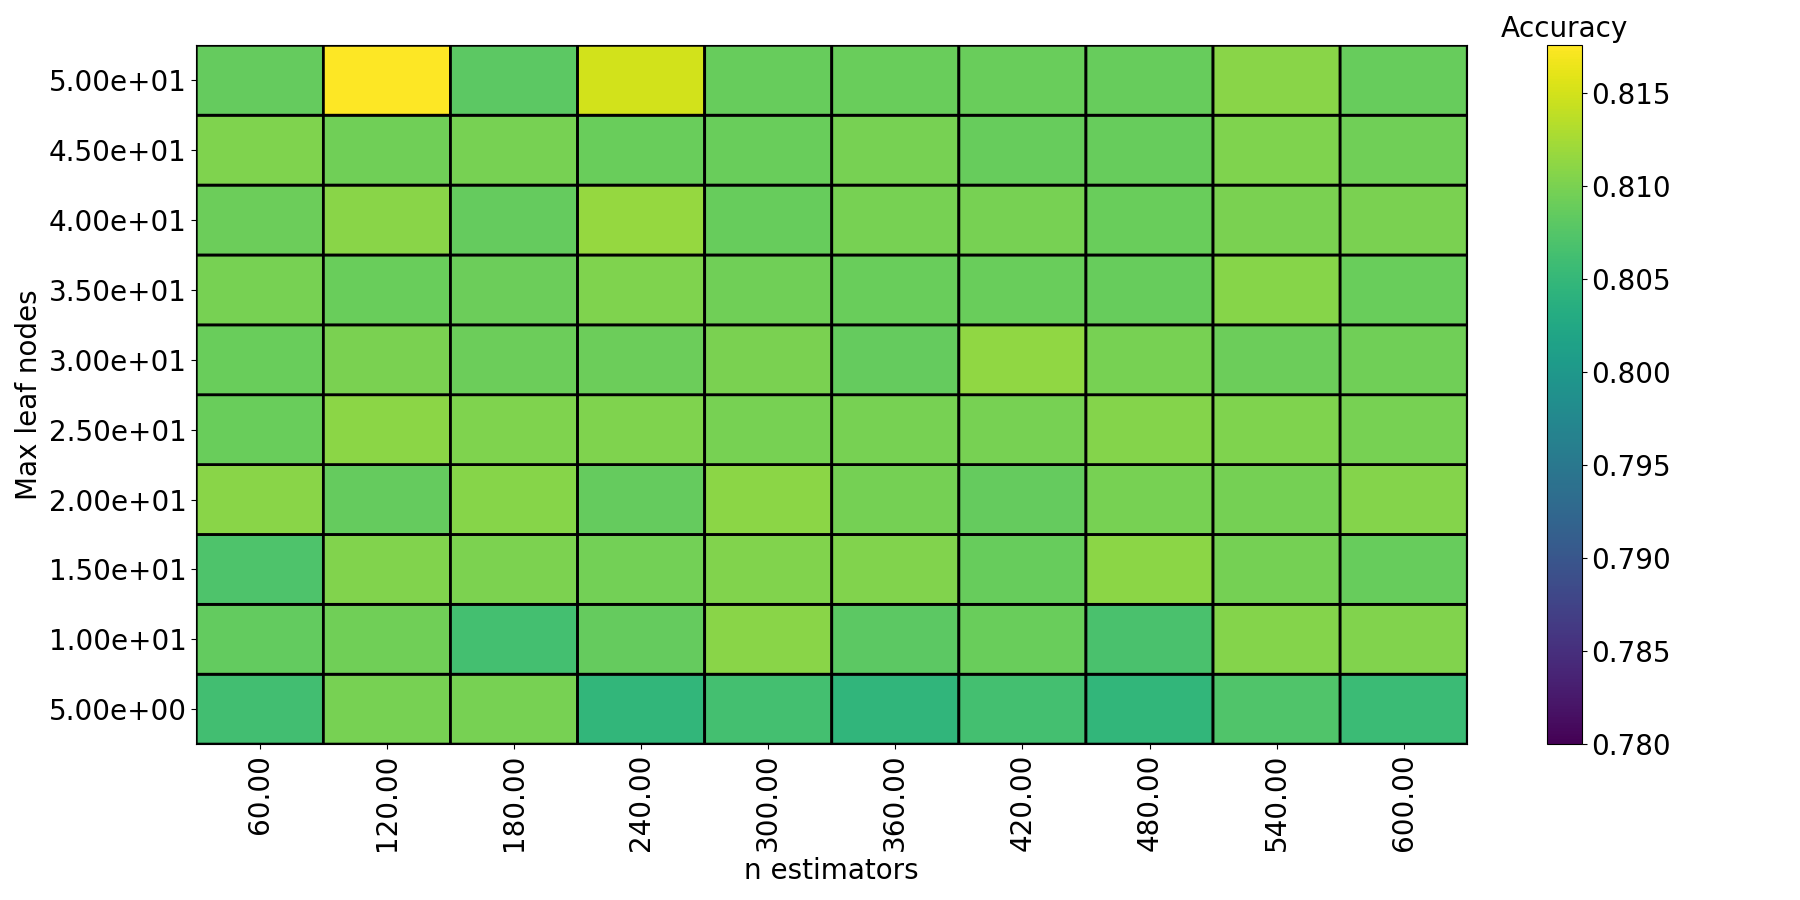
\includegraphics[scale=0.25]{{../figures/-test--nestimators-Maxleafnodes-5.00e+01-Accuracy-mini0.78-maxi0.82}.png}
\caption{A comparison of the Random Forrest accuracy between the parameters}
\label{figR:randomforrest1}
\end{figure}
\begin{figure}[H]
\centering
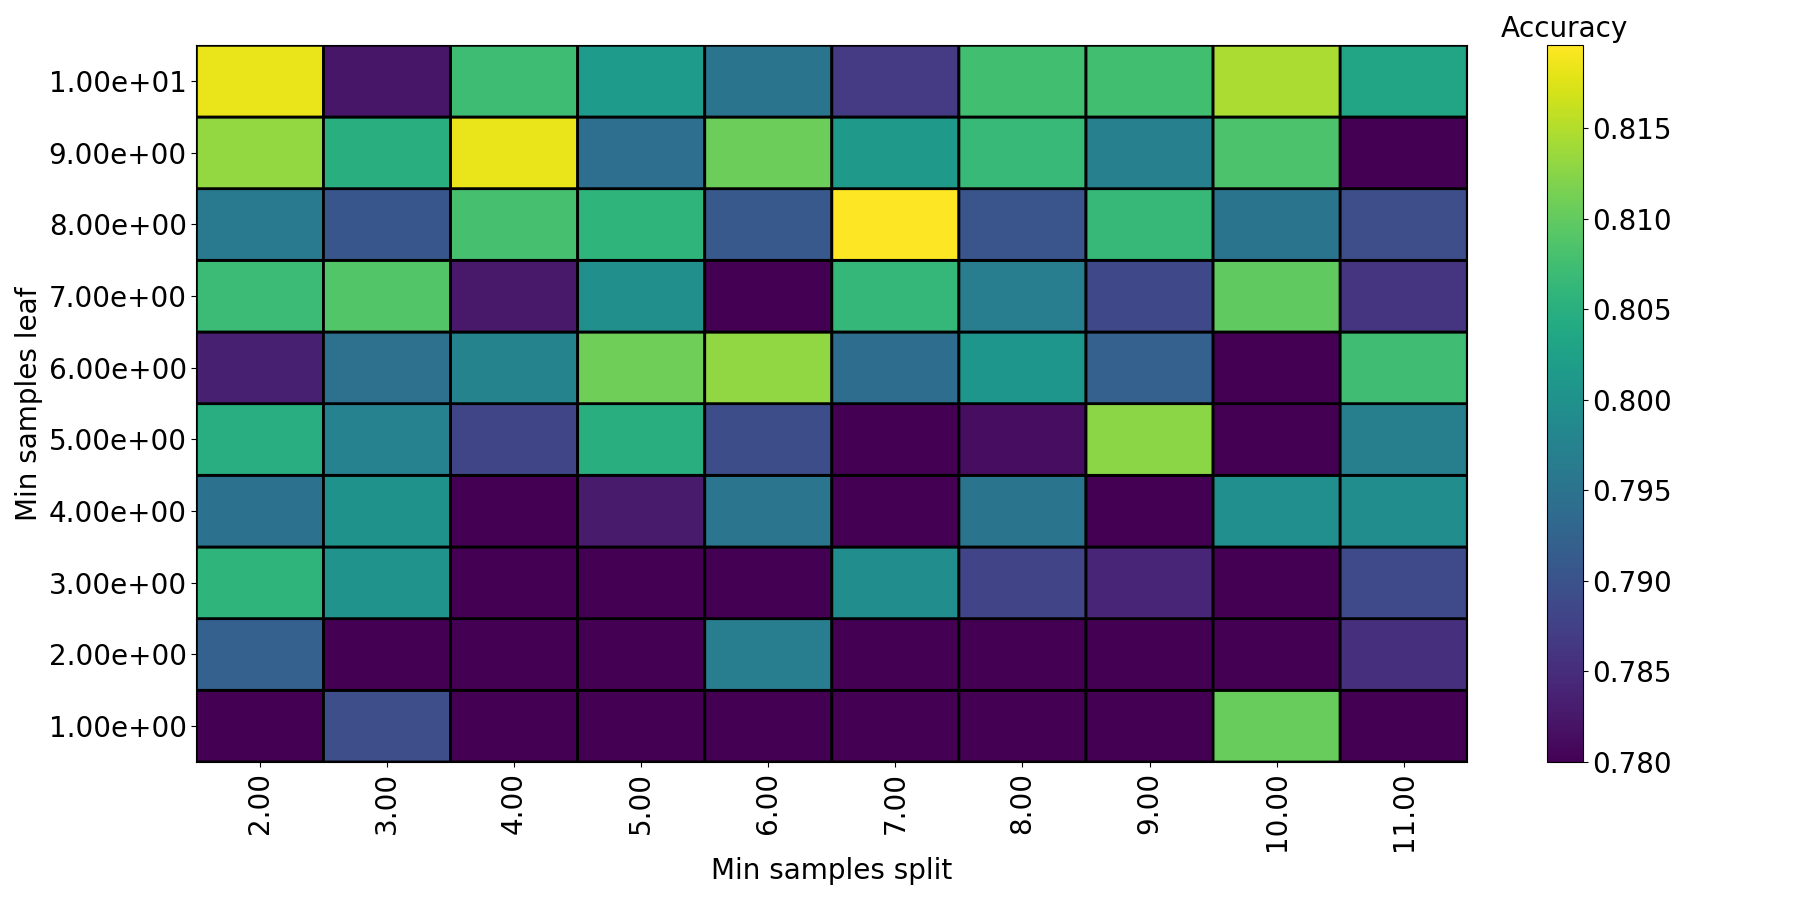
\includegraphics[scale=0.25]{{../figures/-test--Minsamplessplit-Minsamplesleaf-1.00e+01-Accuracy-mini0.78-maxi0.82}.png}
\caption{A comparison of the Random Forrest accuracy between the parameters}
\label{figR:randomforrest2}
\end{figure}
\begin{figure}[H]
\centering
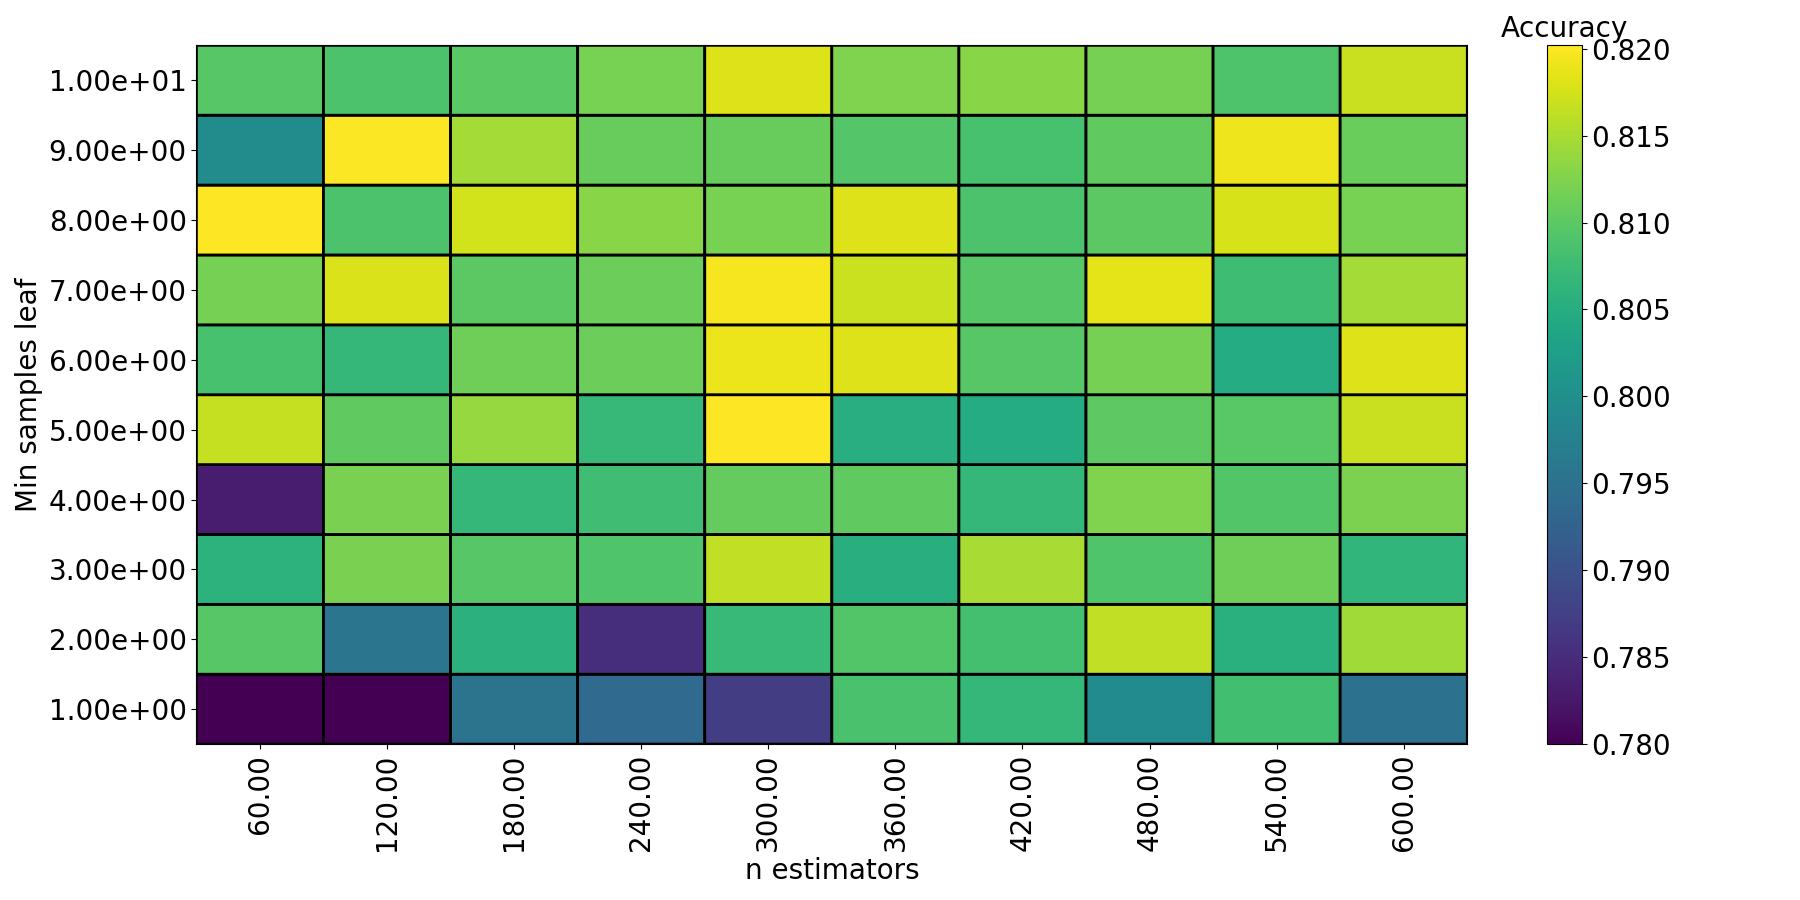
\includegraphics[scale=0.25]{{../figures/-test--nestimators-Minsamplesleaf-1.00e+01-Accuracy-mini0.78-maxi0.82}.png}
\caption{A comparison of the Random Forrest accuracy between the parameters}
\label{figR:randomforrest3}
\end{figure}
\begin{figure}[H]
\centering
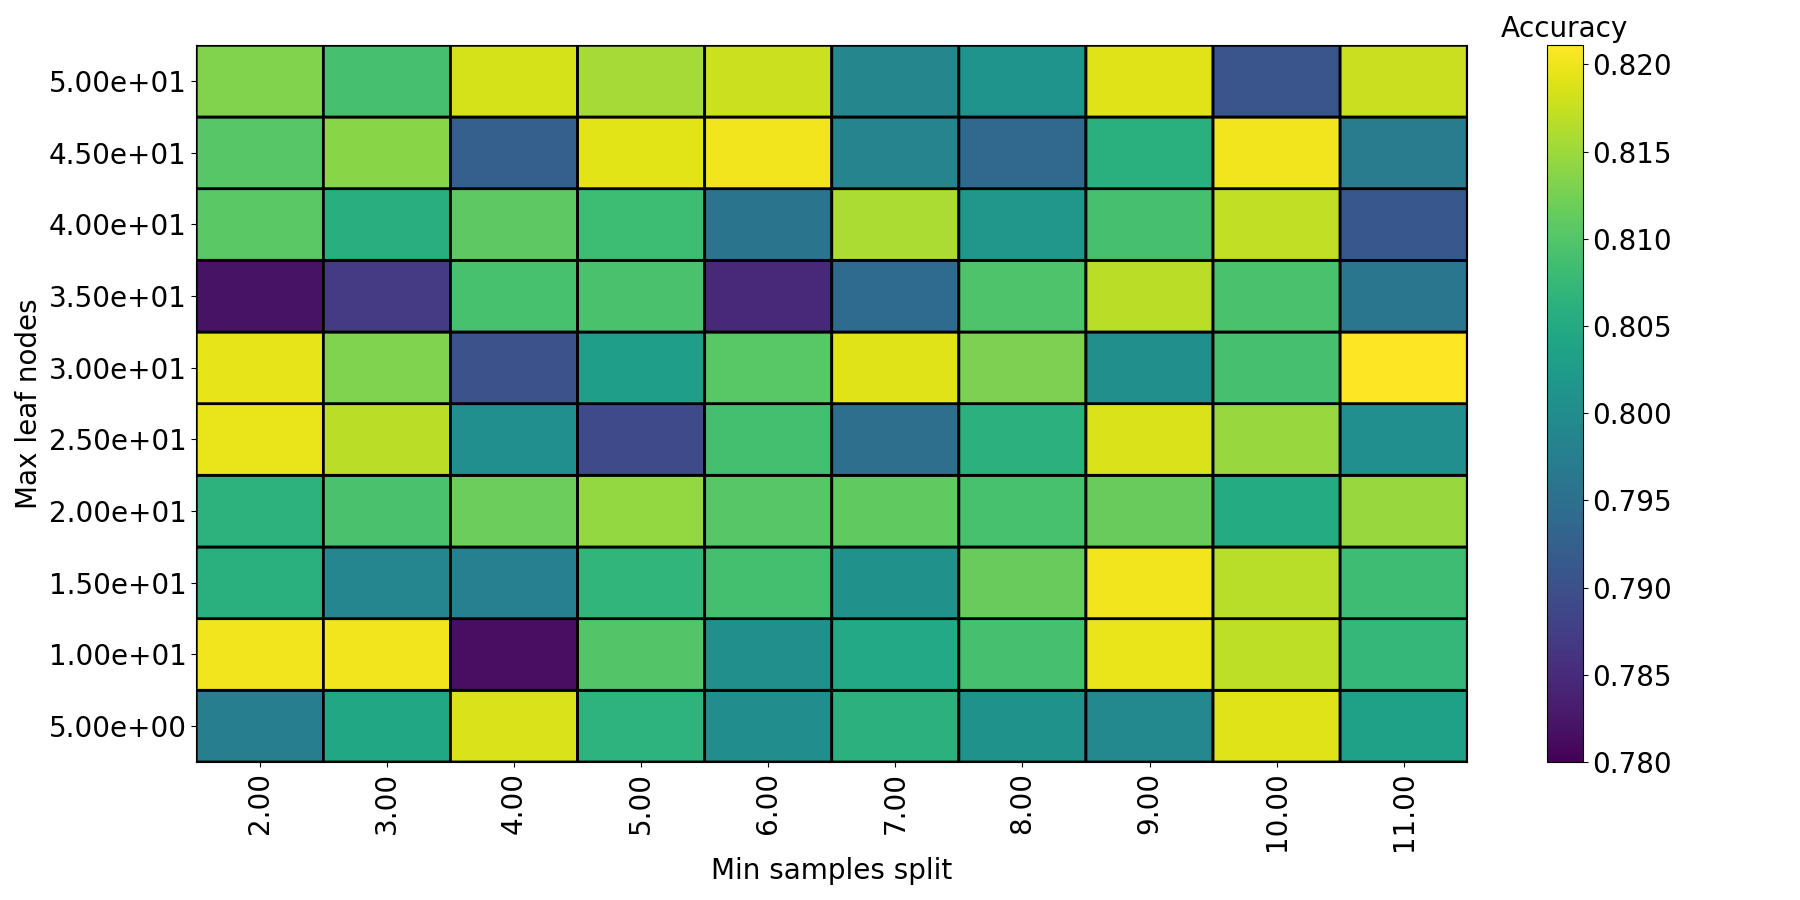
\includegraphics[scale=0.25]{{../figures/-test--Minsamplessplit-Maxleafnodes-5.00e+01-Accuracy-mini0.78-maxi0.82}.png}
\caption{A comparison of the Random Forrest accuracy between the parameters}
\label{figR:randomforrest4}
\end{figure}
As we can see, most plots give little to no information about optimal parameters. Therefore, we do some educated guesses influenced by the color maps and set the parameters to what is found in table \ref{tabR:RFparameters}. These values led to an accuracy of around 81\%, to try and get an even better results, we did trial and error and ended up with the results in \ref{tabR:RFparameters2}. These values were then used to create the gain-chart presented in figure \ref{figR:randomforrest}.
\begin{table}[H]
\centering
\begin{tabular}{c|c}
Parameter & Value \\ \hline
n estimators & 360 \\
Max leaf nodes & 25 \\
Min samples leaf & 6 \\
Min samples split & 9
\end{tabular}
\caption{Estimated optimal parameters for our Random Forrest model}
\label{tabR:RFparameters}
\end{table}
\begin{table}[H]
\centering
\begin{tabular}{c|c}
Parameter & Value \\ \hline
n estimators & 600 \\
Max leaf nodes & 30 \\
Min samples leaf & Default \\
Min samples split & Default
\end{tabular}
\caption{Estimated optimal parameters through trial and error for our Random Forrest model}
\label{tabR:RFparameters2}
\end{table}
\begin{figure}[H]
\centering
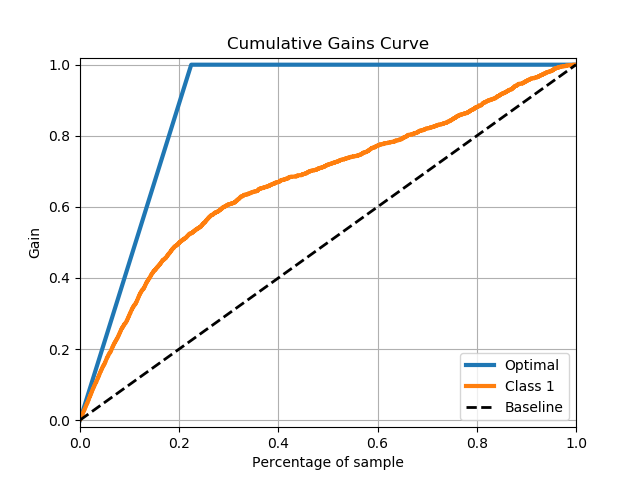
\includegraphics[scale=0.8]{../figures/gain-RF.png}
\caption{Gain chart for our Random Forrest with guessed parameters}
\label{figR:randomforrest}
\end{figure}
All area ratios are presented below in table \ref{tabR:arearatio}:
\begin{table}[H]
\centering
\begin{tabular}{c|c|c}
Method & Test area ratio & Train area ratio \\ \hline
Logistic Regression & 0.43 & 0.46 \\
Neural Network & 0.55 & 0.65 \\
Random Forrest & 0.45 & 0.48 \\ \hline
\end{tabular}
\caption{Area ratio between area of gain curve divided by area of optimal curve. Both areas are measured from above the baseline.}
\label{tabR:arearatio}
\end{table}
\section{Discussion}
As we can see from the results above, the optimal model for these datas are hard to find and we have not performed any better than the article of Yeh et al. \cite{yeh}. There are several reasons behind this. First of all, the data set is small and not well balanced. There are several ways to compensate for this imbalance such as upsampling or downsampling the under represented data class or the over represented class respectively. An attempt was made at upsampling the under represented class by copying the exsisting data for this class, however, this caused a lower accuracy than the standard data set. \\ 
Due to the imbalance of the data set, most classifiers tends to opt for setting all models to guessing the overrepresented class which gives an accuracy of about 77\%. This was initially a challange and effects the whole process even though our current attempts have raised the accuracy to at best 82\%.\\ \\
Furthermore, one could have tuned the models better or set them up differently. This is something that is learned by experience and due to lack of time we were unable to find better parametres than the ones presented in the results. For future works we would like to tune the models even better and enlist the help of more experienced people to help spot the weaknesses of our code. This became especially evident with the random forrest where we are sure there are better solutions, but due to lack of time, we had to resort to trial and error. In the future, we will try to balance the time used on each method better so that the random forrest could have recieved the amount of attention we gave the neural network which was considerably more. \\ \\
The code presented alongside this article realies heavily on libraries and not on homemade code. This approach was chosen due to the fact that we wished to learn how to use the libraries. The in itself has much room for improvement, and in the future we would like to write a better, easier to read and in general more generealized code. \\ \\
Our goal for this paper is to compare different models of classification when given real life data. As we can see from the results, the clear winner is the neural net. However, this is also the model which overfits the data the most. This becomes evident when looking at the difference in training and testing area ratio. It was expected that the random forrest would do as good or even better than the neural net, however, due to time constraints we could never find the parameters which should be tweaked to find the optimal solution. T
he color plots presented in results are sloppy and gives us little information. If we were to find better parameters to compare or found another way to find good parameters, the results would surely improve.\\ \\ 
It is also worth noting that our best accuracies (found in the color plots) were never higher than 83\%. If an model were to guess that all credit card users didn't default, we would have 77\% accuracy as mentioned above. This means that our models are only slightly better than guessing everyone in one category. One way to counter this could have been to penalize guessing the major class wrongly even more or by increasing the weights and biases towards the minor class. If we ever were to visit this problem again, we would try this. \\ \\ 
Furthermore, we can see that our results are on par with those of Yeh et al. \cite{yeh}, which makes us question the nature of their report. Our models are not that good and therefore, neither are theirs. It is interesting to notice the extent of their work, which is formidable, but the quality of their models are not that good. This is even more evident in their predicted probability figures (fig. 8 - 13) which have data points spread all over. It would have been interesting to try and replicate these figures as well, as it would also have given us an oppertunity to calculate R2 and MSE, but this has been left out due to time constraints and is left for future work. Another interesting approach would be to use other activation functions, such as tanh, in the neural net or use MSE as cost function. \\ \\
A final thing to consider when comapring our models are the concept of white and black boxes as presented by Geron on page 172 \cite{Geron}. White box models are intuitively easier to understand and we can understand the logic behind why the model behaves as it does. Black boxes are often great at predicting but even though we can access their inner workings through every step of the way, the process may seem unintuitive and totally at random. It is important to take this into account for two main reasons: Firstly, it is important that you as a programmer have a grasp of what is going on inside your code. Why does the neural net suggest a instead of b. Why do we want to increase the weights in this or that way. Of course, one will never fully understand these black boxes, but it is important to have as much control about the process as possible. Secondly, odds are many programmers will not be programming only for themselves, but have to present their work down the line. For people who do not work with these types of algorithm, an easy explenation to the "magic" that the computer performs may mean the difference between a research grant and not, a job and unemployment etc.
\subsection{Future works}
To summerize our plans for future work, we firmly believe that the random forrest could perform better under different circumstances. In the future we would like to further explore the possibilities behind Random Forrest, preferably under the guidance of someone more experienced. We would also like to find the use regression algorithms on a comparison of predicted probability and actual probability to see if we could find better models than those of Yeh et al. \cite{yeh}. It would also be preferrable to spend more time with each model, trying to improve upon what we have and improve it beyond that of Yeh et al.
\section{Conclusion}
We found that the neural net was our best model even though it was also the model most prone to overfitting. Our area ratios were on par with those of Yeh et al., but not better. The Random Forrest model was expected to do better than it has and it has most likely unused potential in that regard. We leave these improvements for future works.
\bibliography{lib}
\end{document}